\documentclass[10pt,twocolumn,letterpaper]{article}
\usepackage{cvpr}
\usepackage{times}
\usepackage{graphicx}
\usepackage{amsmath}
\usepackage{amssymb}
\usepackage[pagebackref=true,breaklinks=true,colorlinks,bookmarks=false]{hyperref}


\begin{document}
\title{What {\em is} the Best Classifier?\\
       What {\em is} the Best Regressor?}

\maketitle

\begin{abstract}
   This report investigates two questions.
   First, for a given selection of data sets, can we say what
   is the `best' classifier or the `best' regressor in terms
   of good predictions?
   How much does the answer depend on the particular selection of data sets?
   How much does the answer depend on our computational constraints?
   We investigate these questions using data sets from the UCI repository.
   Second, we compare the interpretability of a decision tree
   classifier to that of a convolutional neural network.
   We compare the decision tree visualization
   to `activation maximization', a technique to gain insight into
   the kinds of inputs that deep neural networks respond to.
   Third, are there any other possible ways through which we can improve the performance, considering the computational efficiency as well. 
   Also, after having a brief idea of some of the machine learning concepts, have you tried your knowledge to some other datasets.  
\end{abstract}

%------------------------------------------------------------------------
\section{Introduction}

% DELETE THIS TEXT
%intro with some definition
Supervised learning, one of the category of Machine learning, is further classified as Classification or Regression problem depending upon the dependent variable: categorical or discrete. Before diving into building models, it is necessary to know answers for rising questions: what our data looks like, are there any missing values, does it require scaling/normalization, what are the types of features and are all required in building models and lot more.

Our very first step is to load the data sets in a format easy to interpret. We used pandas for reading and manipulation of data, since it provides hands on features to load data in tabular format (dataframe) and it has built-in methods to summarize the data set. We even checked for class imbalance by printing the frequency of each class for each data set, required for classification. This helps in choosing appropriate metrics for evaluation. 

We made different functions for reading, preprocessing by applying appropriate techniques and splitting the data and process all the files the same way maintaining the consistency through out the project. 

Now that we have clean data, we can feed it to defined classifiers and regressors. We can train on the training data and evaluate the model on the testing data. But, this will lead to overfitting as we are tuning the hyper parameters based on the testing data. Instead, better approach is to use a left out training data called validation data and evaluate model on it. Finally, predict the model on test data. This way we can avoid overfitting the model. We have used hyperparameters selection technique like GridSearchCV and RandomSearchCV.

Once we have best parameters for each model, finally we can fit the model on the best hyperparameters and check for the accuracy. Here, we deal with different metrics based on the application.
% noelty component
We tried to put our knowledge into two other datasets: heart disease dataset and NLP dataset. Our idea is to see whether we can generate/predict the next words from the seen corpus. We have taken a small portion of romeo-juliet play. 
% DELETE THIS TEXT



%------------------------------------------------------------------------
\section{Methodology \& Experimental Results}
This section deals with common strategy applied to both classification and regression problems. 
\newline\textbf{Data loading}: We proposed a common method for classification and regression task to read the whole dataset. 
\textbf{Preprocessing}: In this step, we clean the data by handling missing values. There are many techniques to do so like use the mean value, most frequent value or any value very small or high can be used to fill missing values. Also, there can be columns with categorical features and are required to be in numeric format for most of the Machine learning, though so algorithms like random forest, decision tree can handle them. So, we have used label encoding to convert to numeric values.
\textbf{Splitting}: In this method, we split the dataset in training and testing.  

\subsection{Classification Experiments}
After reading the data, it is necessary to check for the class imbalance especially for classification, that will provide an overview of what metrics to evaluate on.For applications where cost of false negatives is high, recall would be a better metrics to choose. While, in scenarios where cost of false positive is high, precision is the good metrics to evaluate. But, if we need to seek a balance between Precision and Recall, then it is better to go with f1 score. Following section describes methodologies used for each classification dataset including evaluation metrics.
\begin{itemize}
    \item Diabetic Retinopathy: In this data set, it is important that model predicts the true positives accurately, it is not acceptable that any person with daibetic retinopathy is not predicted. Hence, we used recall as an evaluation metric for this data set.    
    \item Default of credit card clients: It is obvious that there will be a very few frauds compared to normal transaction. Hence, this data set is imbalanced. We used recall for evaluation since, it is more important to predict frauds correctly. 
    \item Breast Cancer Wisconsin: Again an imbalanced data set and also cost of true negatives is high so we have used recall. This data set contains '?' as values for a column and so we replaced that with the most frequent value. Also, the target values where 2 and 4 and so we converted to 0 and 1 respectively.  
    \item Australian credit approval: This data set is also imbalanced. Here, cost of false positives is high and so we have used precision as an evaluation metric. 
    \item German credit data: Same as the default credit card data set mentioned above, we used recall.
    \item Steel Plates Faults: This data set also contains imbalanced class. We have used f1 score as an evaluation metric since it depends on both recall and precision.
    \item Adult: This data set contains '?' values and so we replaced it with the most frequent value. Also, values of a column are categorical and so we converted to numeric format using label encoding. 
    \item Yeast: This is multi-class classification problem. Classes are imbalanced and so used f1 score for evaluation. This data set also contains categorical value and so we applied label encoding.
    \item Thoracic Surgery Data: Columns contains categorical data and so we applied label encoding for the numeric conversion. Due to class imbalance, we used f1 score for the evaluation.
    \item Seismic-Bumps: Here, also we have categorical non numeric value and so we applied label encoding. Used f1 score for evaluation.
\end{itemize}
% results
% DELETE THIS TEXT
%Here you'll list the classification data sets (see report guidelines) and explain any methodological
%aspects (models evaluated, evaluation metrics used, {\em etc.}) that are specific to classification.
%Then you should describe your experimental results,
%and reference any relevant figures and/or tables.

\subsection{Regression Experiments}
Following are the datasets used for regression.
% DELETE THIS TEXT
\begin{itemize}
    \item Wine Quality: There were two separate dataset for red and white wine . We analyzed the features and they matched so we merged the two datasets and performed regression on it.
    \item Communities and Crime : The dataset had 127 attributes, out of which 5 were non predictive. So we dropped those attributes. Also, the dataset had many missing values which we handled by replacing them with zeros.
    \item QSAR aquatic toxicity: There was significant difference in the minimum and maximum values for attributes. So, we decided to scale the dataset in quest of better results.
    \item Parkinson Speech : The last column was categorical output. As we're doing regression we dropped that column and used the UPDRS attribute for the regression problem.
    \item Facebook metrics: The dataset had missing values which were replaced by the column mean. Also, one of the feature was 'Date' which was converted using Label Encode.
    \item Bike Sharing: The dataset had attribute 'instant' which was record index and is non predictive. We dropped the attribute and later scaled the dataset.
    \item Student Performance: The dataset contains many categorial features which were in String format. We converted them to integer using Label Encoder. Also, we've performed our analysis using the Portugese language dataset.
    \item Concrete Compressive Strength: Here, also we scaled the dataset due to significant difference in values. 
    \item SGEMM GPU kernel performance: This is one of the biggest dataset in our regression analysis. It had four output attributes of run time in milli-seconds. We  calculated the average time and conerted to single output dataset to be used for regression.
    \item Merck Molecular Activity Challenge: The two Merck Molecular dataset were loaded and cached using npz format. The evaluation metrics used for this problem is same as the original challenge evaluation. We Calculated Pearson Corelation after training on each model and then evaluated both daasets.
\end{itemize}
% results

\subsection{Interpretability Experiments}

% DELETE THIS TEXT
This section is based on results observed for CIFAR 10 dataset. Data set includes 10 classes. It is divided into training and testing samples. It is divided into training and testing files. Dataset is in byte format and so we made a method that reads, as described in the UCI repository for this dataset, both training and testing data at once. What we observed seen some images is they are taken centering on the targets. That is, there is less noise in the dataset. The images are in color channels with values in range (0,255) for each 3 channel. So, before feeding the data for decision tree or neural network we scaled it. In case of decision tree we used MinMaxScaler while in case of neural network we divide each value by 255 to rescale in range (0,1). Results obtained were very interesting. In case of decision tree, we save the final tree image since it was too large to be interpreted easily. It is interesting to see how a class get further classified. In case of neural network, we ploted convolutional layer and linear layer to see how these layers look like. Black portion in the image is due to padding. We can easily identify the linear leayer as it is fully connected layer and so we can see a fully grey image. After training the network, we plotted the activation of an image. And it is visible from the figure how edges are smoothed in each layer. These transformations are based on the filters we applied. The results can be improved by applying transformations on the images.
\begin{figure}
   \begin{center}
   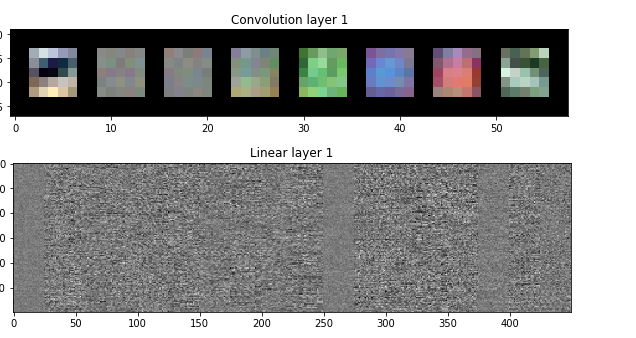
\includegraphics[width=15cm,height=5cm,keepaspectratio]{layer1.png}
   \end{center}
      \caption{Convolution and Liner layer\label{activation}}
\end{figure}

\begin{figure}
   \begin{center}
   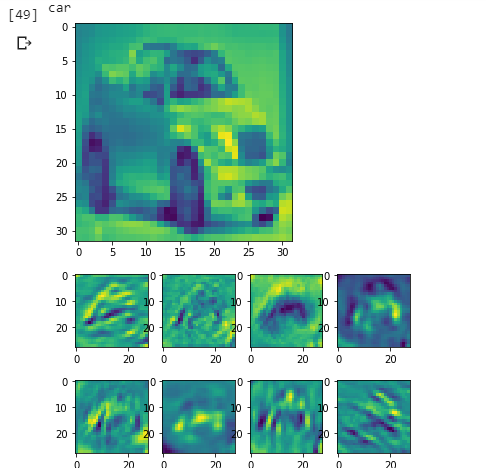
\includegraphics[width=15cm,height=5cm,keepaspectratio]{activation.png}
   \end{center}
      \caption{Activation of car\label{activation}}
\end{figure}



% add figures from the experiments


%------------------------------------------------------------------------

\section{Conclusions}

% DELETE THIS TEXT
Here you should summarize your thoughts on the questions asked in the abstract.
\newline After running models on twenty different datasets, we can conclude that we cannot give the title of best classifier or best regressor to any one model. Different techniques respond differently to different datasets. A number of things like size of dataset, number of features and type of values in the data. Also, we could see that there is a clear trade off between accuracy and computational complexities and time taken to train the model.
\newlineAfter thorough analysis, for Classification, we can say that ensembles are clear winners. Random Forest and AdaBoost performed much better on an average against rest of their competitors. Multiple estimators in ensembles kicks out the uncertainty and arbitrariness of models like decision tree. Also, Logistic Regression gives surprisingly good results. It's performance of significantly increases after hyper-parameter search. It works best when working with binary data and also takes significantly less time to train compared to ensembles. One more observation from our analysis is that Logistic Regression didn't over-fit. Support Vector Machines give decent results but take a lot of time when number of features are more. Neural Networks can give great result, but requires fine tuning the hidden layers and units. This can be a very difficult task for an amateur in the field. But when given more time to train they can give state-of-the-art performance especially for images. Gaussian Naive Bayes result were very bad. The biggest reason can be the  assumptions of independence upon which it works. But if those assumptions hold true, it can give very good results with very less training data.

\newline In case of Regression, Random Forest was once again significantly ahead compared to it's competitors. Also in case of data that had a linear trend, Linear Regression and Support Vector Regressor with Linear kernel performed really great. Linear Regression is definitely go-to regression technique when the data is in linear shape. But, SVM took a lot of time to train, especially when features were more. In our experiments we also used Ridge Regression which is same as Linear Regression but has an added feature of regularization which allows us to fine tune the results. However, in almost all datasets, even after regularization there wasn't significant increase in the scores. Decision Tree Regression gave good result but didn't generalize well so the test results were not good enough. Thanks to ensembles we can deal with this randomness. AdaBoost tries to turn a weak learner into a strong learner. It gave decent results. Gaussian Process Regressor performed the worst. It memorized all the training data so gave perfect training accuracy almost always, but when it comes to predicting, it failed. It also crashed when the dataset was big like in case of SGEMM GPU Kernel dataset. 


So, if a colleague of mine were to download similar datasets like the ones in this study, Random Forest is definitely a go to. With exhaustive search it can give great result. In case of lack of good computational resources Logistic Regression is the first one a person should try.
\newline In the interpretability section, neural network has an accuracy around 59\%. We have used a model with 2 convolutional layers followed by max pool layer and then linear layres. With this little complex layers we have seen interesting patterns that model makes while classifying. We can increase the accuracy by adding more layers to the network but have to keep in mind that more complexity leads to overfitting. We can instead use transformations like rotating the images by some degree, because it is possible that model has learnt how a dog looks like when standing, but what happens when we have an image of sleeping dog! Hence, by applying such data agumnetation techniques we can approve the performance.

After going through multiple medical related datasets in this study, we were inspired to use one more. One of the novelty component was working with heart disease dataset for classification problem. All the models performed really well and gave results in high 80s. In regression we tried to regularize Linear Regression and use Ridge Regression in the hope of getting better scores. There wasn't significant increase in the results even after searching through parameters.

 Another novelty component, NLP, the results were quite justified. We gave as an input some words of the play and made predictions on the next most 10 frequent words. You can of course change this to your choice. We have used a very small dataset and so our accuracy is not good but is also not the worst. 

 At last we can conclude that there are pros and cons of using any technique. With better understanding of the data, one can figure out which model could work best.
 
 \section{Overview of project code and data}
Please find all information in README.txt file in the project folder. More Plots are present in the Plot folder. Exhaustive result and best model details are in XLS files in the project  folder.
\newpage

\begin{figure}
   \begin{center}
   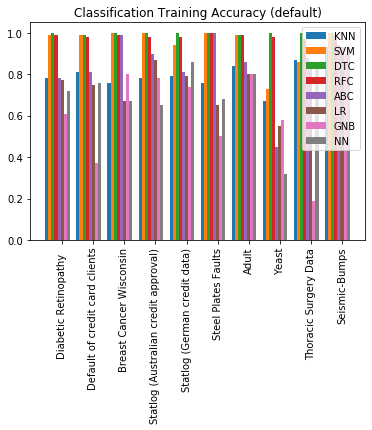
\includegraphics[width=15cm,height=5cm,keepaspectratio]{Classification Training Accuracy (default).png}
   \end{center}
      \caption{Classification on training accuracy\label{Classification training accuracy}}
\end{figure}

\begin{figure}
   \begin{center}
   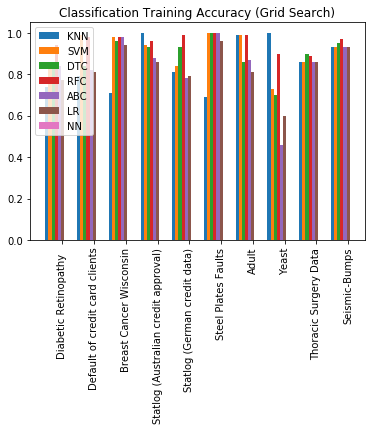
\includegraphics[width=15cm,height=5cm,keepaspectratio]{Classification Training Accuracy (Grid Search).png}
   \end{center}
      \caption{Classification on training accuracy(Grid Search)\label{Classification training accuracy}}
\end{figure}



\begin{figure}
   \begin{center}
   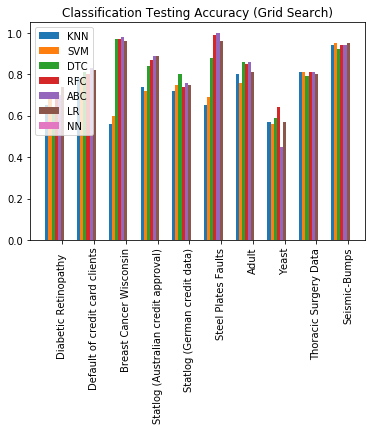
\includegraphics[width=15cm,height=5cm,keepaspectratio]{Classification Testing Accuracy (Grid Search).png}
   \end{center}
      \caption{Classification on testing accuracy (Grid Search)\label{Classification testing accuracy}}
\end{figure}


\begin{figure}
   \begin{center}
   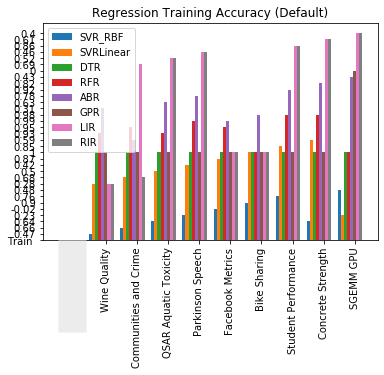
\includegraphics[width=15cm,height=5cm,keepaspectratio]{Regression Training Accuracy (Default).png}
   \end{center}
      \caption{Regression on training accuracy\label{Regression training accuracy}}
\end{figure}

\begin{figure}
   \begin{center}
   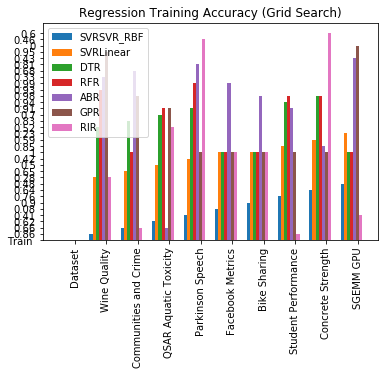
\includegraphics[width=15cm,height=5cm,keepaspectratio]{Regression Training Accuracy (Grid Search).png}
   \end{center}
      \caption{Regression on training accuracy(Grid Accuracy)\label{Regression training accuracy}}
\end{figure}
\begin{figure}
   \begin{center}
   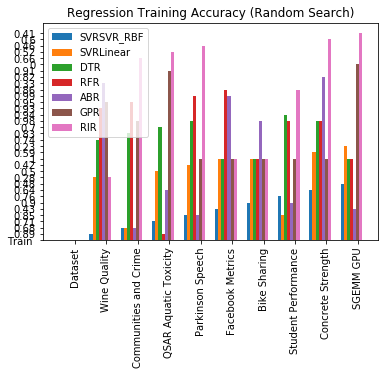
\includegraphics[width=15cm,height=5cm,keepaspectratio]{Regression Training Accuracy (Random Search).png}
   \end{center}
      \caption{Regression on training accuracy (Random Search)\label{Regression training accuracy}}
\end{figure}
\begin{figure}
   \begin{center}
   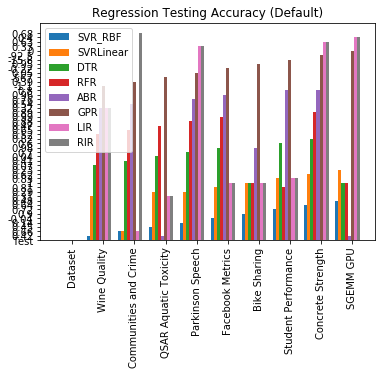
\includegraphics[width=15cm,height=5cm,keepaspectratio]{Regression Testing Accuracy (Default).png}
   \end{center}
      \caption{Regression on testing accuracy\label{Regression testing accuracy}}
\end{figure}

\begin{figure}
   \begin{center}
   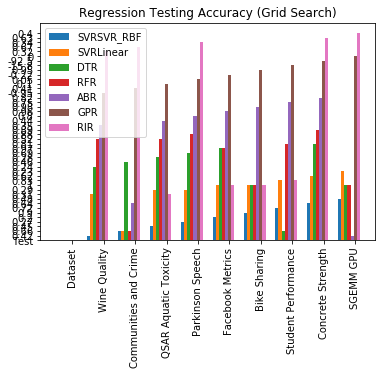
\includegraphics[width=15cm,height=5cm,keepaspectratio]{Regression Testing Accuracy (Grid Search).png}
   \end{center}
      \caption{Regression on testing accuracy (Grid Search)\label{Regression testing accuracy}}
\end{figure}

\begin{figure}
   \begin{center}
   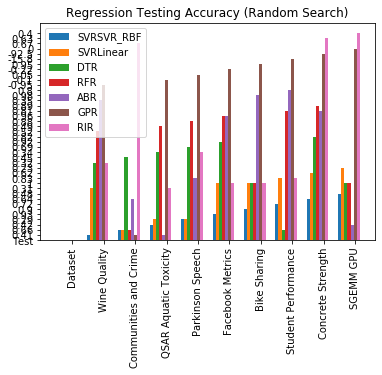
\includegraphics[width=15cm,height=5cm,keepaspectratio]{Regression Testing Accuracy (Random Search).png}
   \end{center}
      \caption{Regression on testing accuracy (Random Search)\label{Regression testing accuracy}}
\end{figure}
\newpage

\appendix



%-------------------------------------------------------------------------





\end{document}
